\chapter{Recurrent Neural Network}
Il problema delle CNNs è che essenzialmente \textbf{non riescono a performare 
quando sono applicate a task che hanno a che fare con sequenze di qualsiasi tipo}.
Alcuni esempi di task di questo tipo sono:
\begin{itemize}
   \item \textbf{speech recognition}, l'input è una traccia audio e 
   l'output è la trascrizione (quindi la sequenza di parole) corrispondente; 
   \item \textbf{music generation}, in input non abbiamo niente, in output 
   produce una sequenza di note;
   \item \textbf{sentiment classification}, in input abbiamo una frase, 
   quindi una sequenza di parole, in output produciamo un valore che rappresenta un sentimento;
   \item \textbf{DNA sequence analysis}, in input abbiamo una sequenza di "", 
   in output abbiamo una sottosequenza che corrisponde ad una proteina;
   \item \textbf{machine translation}, in input abbiamo una sequenza di parole in una data lingua, 
   in output produciamo la sequenza di parole in un'altra lingua, corrispondente alla
   traduzione della fra in input;
   \item \textbf{video activity recognition}, in input abbiamo una sequenza frames, 
   l'output è la loro classificazione;
   \item \textbf{name entity recognition}, in input abbiamo una sequenza di parole, 
   in output etichettiamo alcune (o tutte) le parole;
   \item \textbf{words prediction}, in input abbiamo una sequenza di parole, in output 
   abbiamo una delle possibili parole che continuano la sequenza iniziale.
\end{itemize}
\newpage
Ma perchè le reti neurali standard (come il multilayer perceptron)
non possono risolvere questi problemi di traduzione automatica? 
Prendiamone in esame uno: abbiamo in input una sequenza di parole che 
rappresentano una parola in francese e utilizziamo un mlp per risolvere il 
task di trduzione in inglese. Quale potrebbe essere il problema, o i problemi,
nell'utilizzo di un approccio di questo tipo alla risoluzione di un task di
machine translation? Sono diversi:
\begin{itemize}
   \item \textbf{le associazioni da fare sono troppe}, nella slide sotto, ogni $x$ in input rappresenta una
   parola della frase da tradurre e ogni parola va mappata sulla corretta parola tradotta;
   \item \textbf{bisogna tenere conto del contesto}, per una corretta traduzione di una parola,
   bisogna obbligatoriamente tenere conto delle parole che la precedono e seguono (es. "any");
   \item \textbf{input e output potrebbero avere lunghezza differente}, non è detto che una lingua da 
   tradurre utilizzi lo stesso numero di parole della lingua tradotta;
   \item  \textbf{non è possibile condividere feature apprese in posizioni diverse}, il modello tratta gli 
   input in maniera completamente separata ed individuale.
\end{itemize}
\begin{figure}[!h]
   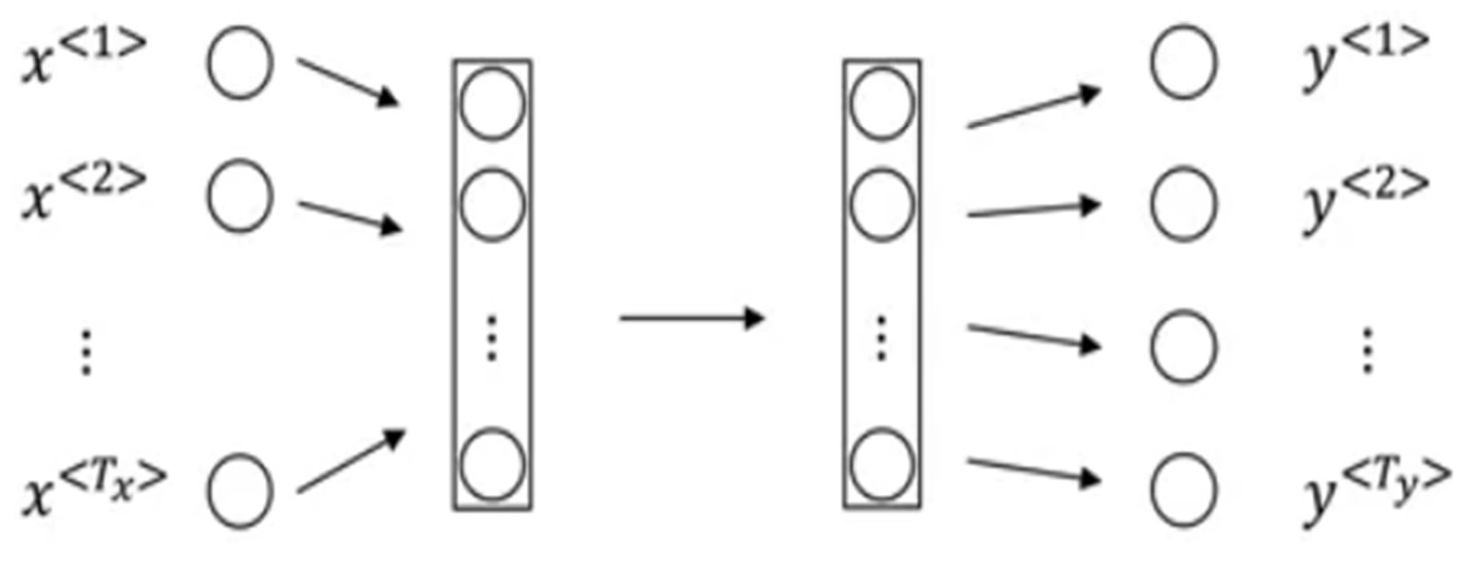
\includegraphics[scale=.5]{images/rnn/mlp.png}
   \centering
\end{figure}
\newpage
\section{Le reti neurali ricorrenti}
Quindi essenzialmente il motivo per cui non siamo reti neurali standard, come mlp, per risolvere
problemi di machine translation è che \textbf{non sono state pensate per questi task, quindi non
riescono a risolvere i problemi legati ad essi}. L'architettura appositamente pensata risolverli è la
\textbf{recurrent neural network (rnn)}, disegnata per ricevere e produrre sequenze. Tra l'input 
$x$ e l'output $y$ (che è la traduzione) c'è un \textbf{layer di hidden unit}. 
Ogni input è quindi trattato in questo modo, in maniera ricorrente da una parola alla successiva. 
\textbf{Tra una rappresentazione e l'altra si tiene anche conto dell'attivazione della precedente unità}. 
Quindi se all'inizio, per la prima parola, il processo tiene conto solo dell'input, per ogni parola successiva
alla prima, all'iterazione successiva viene passato in input non solo la parola che deve processare (ricordiamo
che faccaimo un'iterazione per ogni parola) ma anche il valore di attivazione del layer precedente. Segue
la rappresentazione della rete \textit{unrolled}, cioè in maniera esplicita.
\begin{figure}[!h]
   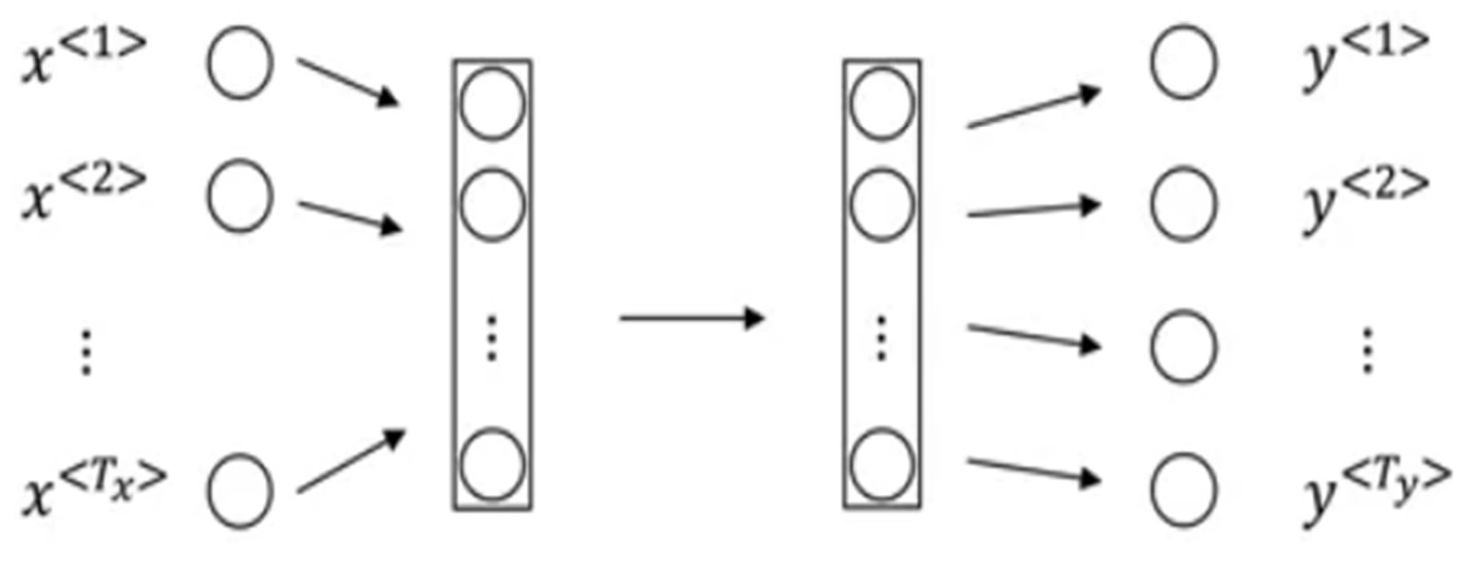
\includegraphics[scale=.5]{images/rnn/mlp.png}
   \centering
\end{figure}


Esattamente la stessa rete può essere rappresentata in maniera più compatta nella sua versione \textit{rolled}.
\textbf{slide 17}: che può essere rappresentata anche nella sua versione più compatta come nella slide
\begin{figure}[!h]
   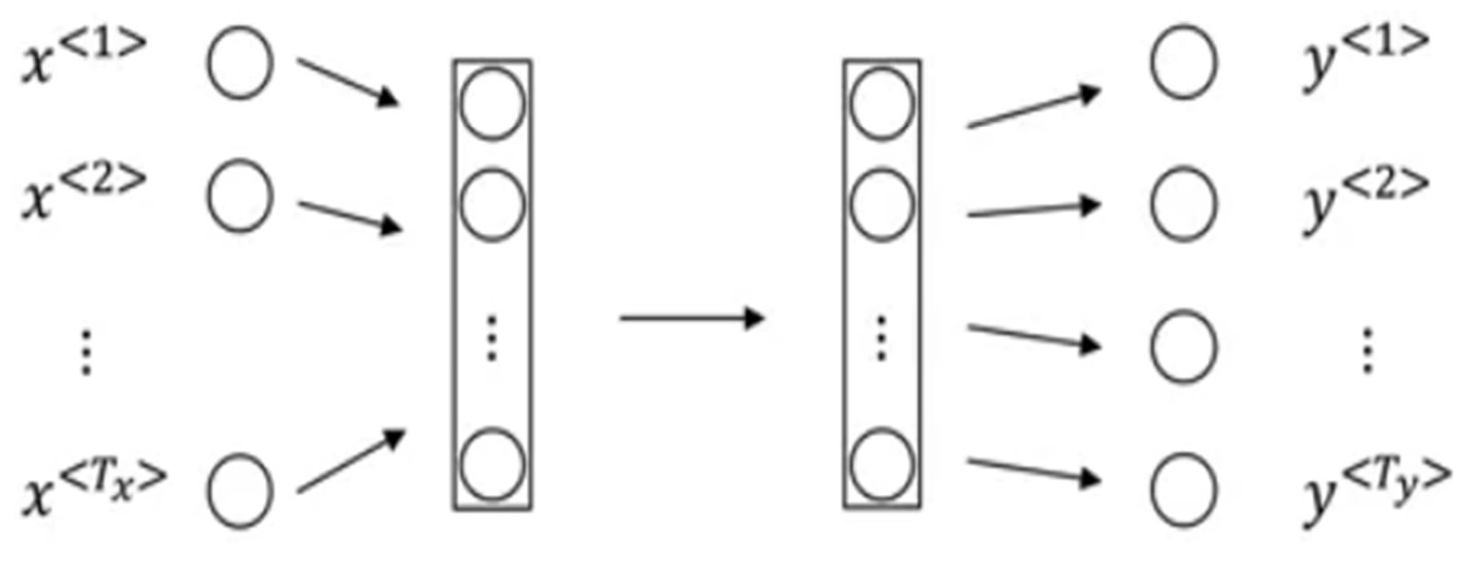
\includegraphics[scale=.5]{images/rnn/mlp.png}
   \centering
\end{figure}


Quindi essenzialmente vegono calcolati due valori: output $y$ e valore di attivazione $a$. Per la prima
iterazione abbiamo $a^{<0>}=\text{zero vector}$.
\begin{equation}
   a^{<n>}=g(W_{ax}x^{<n>}+b_a),
\end{equation}
\begin{equation}
   \hat{y}^{<n>}=g'(W_{ay}a^{<n>}+b_y).
\end{equation}
La \textit{rolled} rappresentation mostra chiaramente che \textbf{i pesi sono condivisi}.
Ovviamente nei veri language models abbiamo delle rappresnetazioni molto più sofisticate, 
\textbf{gli embeddings}. Normalmente queste rnn sono trainate con \textbf{backpropagation},
dove viene calcolato l'errore ad ogni iterazione e questa serie di errori è 
poi utilizzata per il calcolo dell'errore finale. Questo viene poi utilizzato come 
loss function per gradiente dell'algoritmo di backpropagation. 
I due più grandi limiti di queste rnn sono: \textbf{vanishing or exploding gradient} e 
il fatto che \textbf{non sono efficienti nel catturare long distance dependencies}.
\newpage
Per riuscire a catturare questo tipo di dipendenze abbiamo bisogno di un qualche tipo di \textbf{memoria}.
Alcune esempi sono:
\begin{itemize}
   \item \textit{the \textbf{cat}, that had alreay eaten a lot, \textbf{was} full};
   \item \textit{I grew up in France $\dots$ I speak fluent}.
\end{itemize}
\textbf{L'architettura che abbiamo analizzato finora non riesce a risolvere questo problema.}
\subsection{Long Short Term Memory}
Di nuovo, anche questa architettura è stata pensata appositamente per questo problema.
Nella \textbf{long short term memory (lsmt)} le \textbf{lstm cell sostituiscono gli hidden level} 
delle rnn semplici. Ogni cella riceve un input al tempo $t$ ed in seguito produce un output. 
Qual è la differenza rispetto a prima? L'idea che in lstm abbiamo dei \textbf{gates che 
modulano il tipo di informazione che si propaga}. Le celle hanno una \textbf{memoria interna},
cioè un vettore di memoria, che essenzialmente corrisponde all'attivazione dell'hidden layer. 
Questo viene modificato dai vari gate. 
\begin{figure}[!h]
   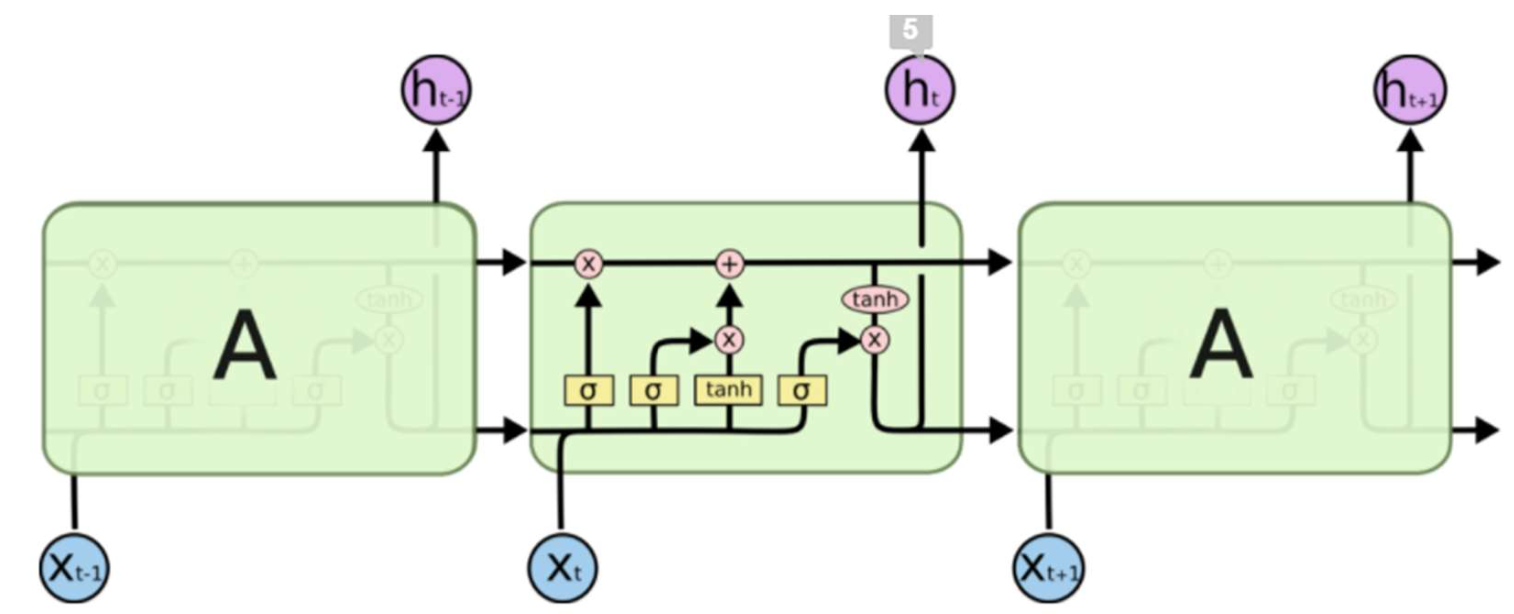
\includegraphics[scale=.5]{images/rnn/lstm.png}
   \centering
\end{figure}


I tre elementi fondamentali sono:
\begin{itemize}
   \item \textbf{lo stato della cellula};
   \item \textbf{il forget gate};
   \item \textbf{l'input gate};
   \item \textbf{l'output gate}.
\end{itemize}
Lo \textbf{stato della cellula} è rappresentato dalla linea orizzontale nella parte alta del diagramma.
Trasporta le informazioni lungo l'intera catena, con solo alcune interazioni lineari minori. Questa 
architettura ha la capacità di rimuovere o aggiungere informazioni allo stato 
della cellula, attentamente regolata da strutture chiamate porte.
\begin{figure}[!h]
   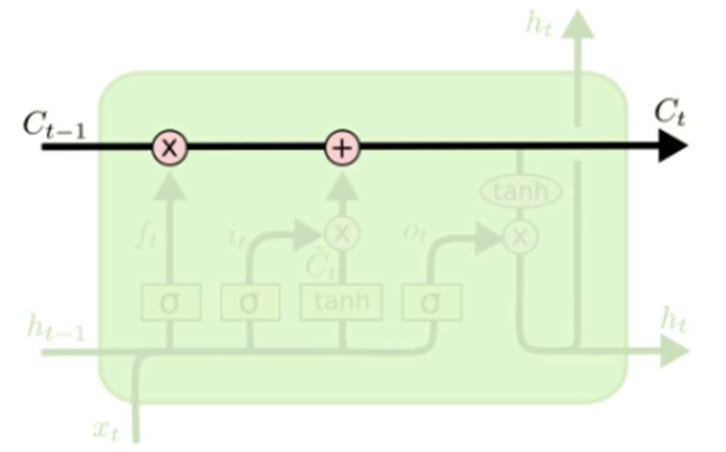
\includegraphics[scale=.5]{images/rnn/cell_state.png}
   \centering
\end{figure}
\newpage
Il \textbf{forget gate} ha il compito di \textbf{eliminare le informazioni}. Sostanzialmente si tratta
di un vettore di valori tra $0$ e $1$, il quale decide quali informazioni tenere e quali
scartare. Moltiplicando le informazioni con una matrice dei pesi si ottiene appunto
un vettore di valori tra $0$ e $1$ che ha la stessa dimensione del cell state ed è
utilizzato per modificarlo. Dove abbiamo $0$ l'informazione viene scartata, 
dove abbiamo $1$ viene propagata.
\begin{figure}[!h]
   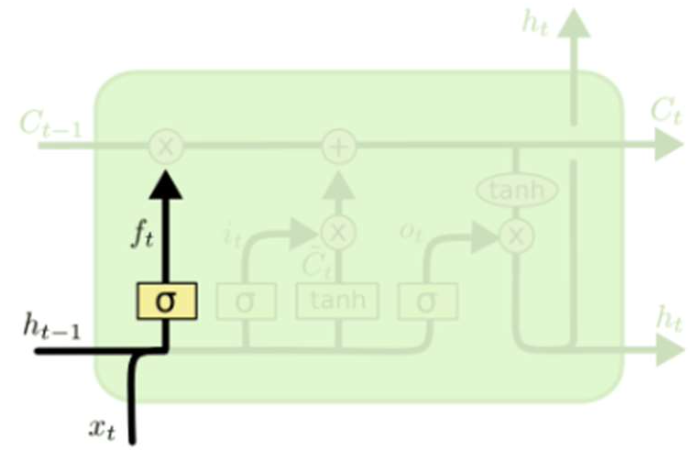
\includegraphics[scale=.5]{images/rnn/forget_gate.png}
   \centering
\end{figure}


\textbf{Facciamo un esempio}: sia la matrice dei pesi

\[ W_f=
\begin{bmatrix}
    1& 1& 1 & -10 \\
    1& 1& 2 & -10 
\end{bmatrix}
\]
e sia $\sigma$
\begin{equation}
   \begin{cases} 
      \sigma=1, & \text{se informazione}>0 \\ 
      \sigma=0, & \text{altrimenti}.
   \end{cases}
\end{equation}
Siano poi $b_f=0$ e $[h_{t-1},x_t]=[1,1,0,1]$ (supponiamo che $x_t=[0,1]$ codifichi "."). Allora avremmo:
\begin{equation}
   f_T=[0,0].
\end{equation}
Intuitivamente (ed informalmente) "." cancellerà tutto da $C_{t-1}$. 
\newline
L'\textbf{input gate} ha invece il compito di \textbf{aggiungere le informazioni}.
\begin{figure}[!h]
   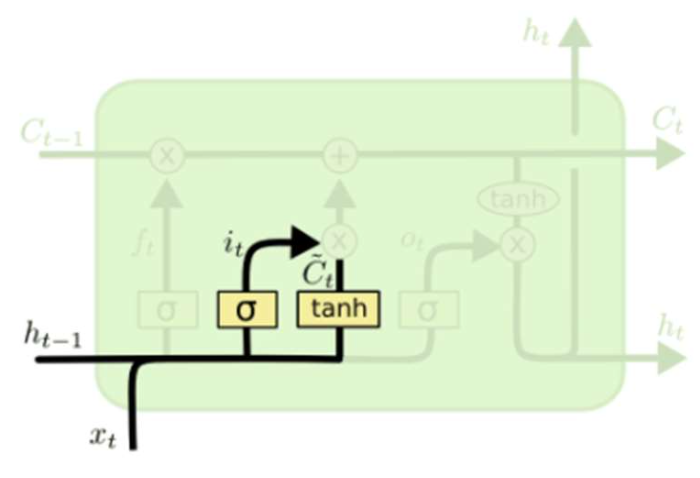
\includegraphics[scale=.5]{images/rnn/input_gate.png}
   \centering
\end{figure}


L'\textbf{output gate} decide infine \textbf{quali informazioni mandare 
al prossimo layer}.
\begin{figure}[!h]
   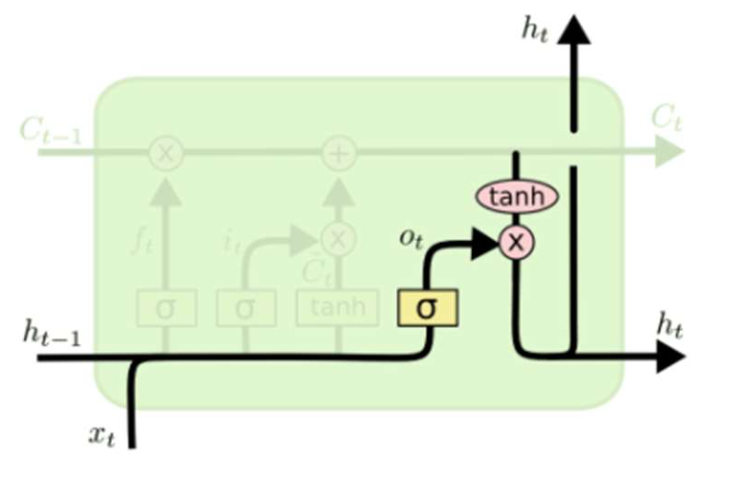
\includegraphics[scale=.5]{images/rnn/output_gate.png}
   \centering
\end{figure}
\newpage
Quindi sostanzialmente ciò che differenzia le CNNs dalle RNN è la presenza, in queste ultime,
delle cell units. Il primo gate, il forget gate, modula il cell state scartando alcune informazioni;
il secondo gate, l'input gate, fa l'opposto, ciò aggiunge informazioni alla memoria corrente (il 
cell state, il corrispondente dell'attivazione); il terzo gate, l'output gate manda le informazioni
al layer successivo. Questo è il modo in cui vengono gestite le long term dependencies.
\newline
\newline
In realtà abbiamo visto una storia \textit{antropomorfizzata} dei gates:
nella realtà non sono fatti a mano e il processo non è ovviamente così chiaro. Un esempio di applicazione 
reale è quella della seguente immagine. 
\begin{figure}[!h]
   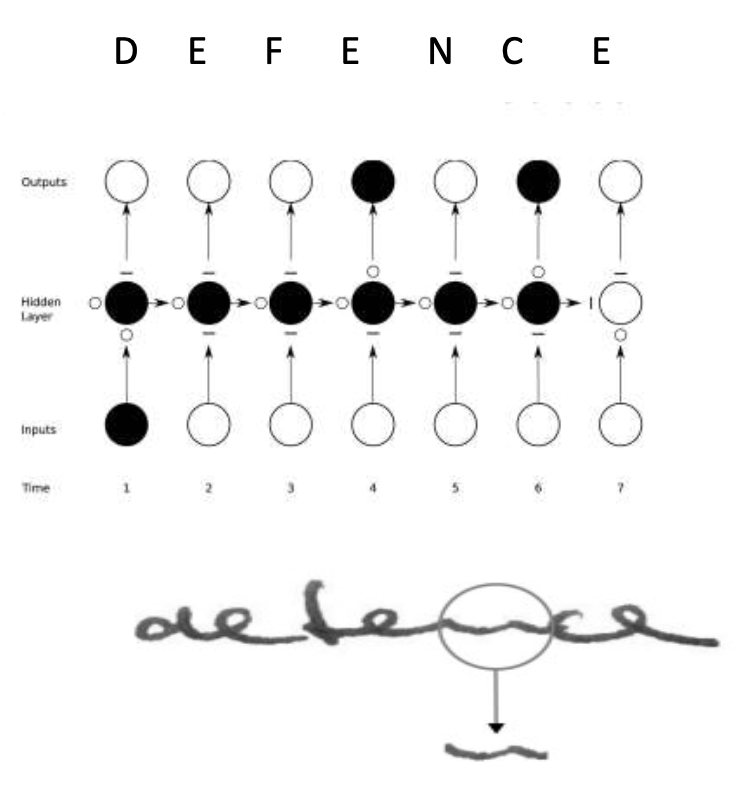
\includegraphics[scale=.5]{images/rnn/real_app.png}
   \centering
\end{figure}


Il modello riceve in input una sequenze di caratteri scritti a mano e 
restituisce in output la sequenza dei caratteri corrispondenti. 
Ovviamente l'interpretazione dei singoli caratteri dipende anche dal contesto. 
La rete è composta da in input layer, un lsmt layer e un output layer.
\newline
\newline
Un altro tipo di architettura lsmt è il tipo \textbf{stacked}. 
In generale offre prestazioni molto migliori rispetto ad un solo layer di lsmt.
\begin{figure}[!h]
   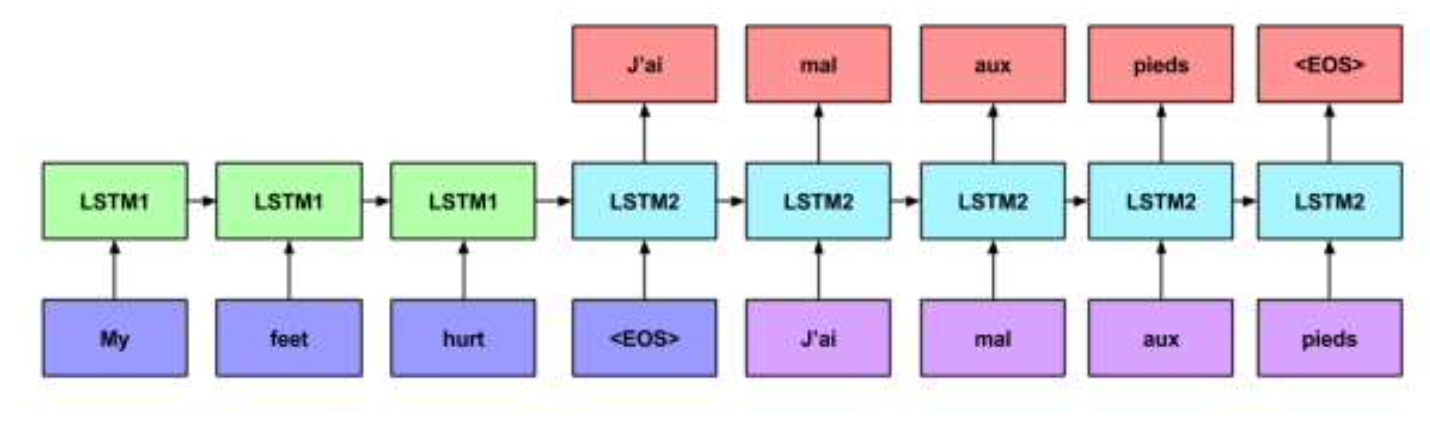
\includegraphics[scale=.5]{images/rnn/stack_lsmt.png}
   \centering
\end{figure}